\chapter{Application:anisotropic shape distribution}

\section{Overview}\label{sec:svg-overview}
  This paper presents an automatic method for computing anisotropic 2D shape distribution on arbitrary 2-manifold meshes.
  Our method allows the user to specify the direction as well as the density of the distribution.
  Using a pre-computed lookup table, our method can efficiently detect collision among the to-be-distributed shapes on 3D meshes.
  In contrast to the existing approaches, which usually assume the 2D objects are isotropic and of simple geometry,
  our method applies for complex 2D objects and can guarantee the distribution is conflict-free, which is a critical constraint in many applications.
  It is able to compute multi-class shape distribution and support maximal distribution so that no additional shapes can be inserted.
  Moreover, it can also be implemented in parallel.
  Our method does not require global parameterization of the input 3D mesh.
  Instead, it compute local parameterization on the fly using geodesic polar coordinates.
  Thanks to the recent breakthrough in geodesic computation, the local parameterization can be computed at little cost.
  As a result, our method can be applied to models of complicated geometry and topology.
  Experimental results on a wide range of 3D models and 2D anisotropic shapes demonstrate the good performance as well as the effectiveness of our method.

\begin{figure}[htbp]
  \centering
  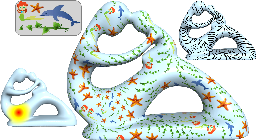
\includegraphics[width=0.8\textwidth]{figs/asd/fertility_multiclass_density.png}\\
  \caption{Given a 3D triangle mesh $M$ and a set of 2D anisotropic shapes,
  the user first specifies a vector field for directional control (see the top-right inset) and a scalar field for density control (see the bottom-left inset).
  Then our method automatically distributes the given 2D shapes onto $M$, satisfying the user-specified directional and density constraints.
  It takes only 2.9 seconds to distribute 4 classes of objects on this 400K-face Fertility model.
  Timing was measured on a quad-core CPU at 2.66GHz.
  }
  \label{fig:teaser}
\end{figure}

\section{Introduction}

  Sampling has a wide range of applications in computer graphics, such as geometry processing, texturing, and rendering.
  Among many sampling techniques, blue noise is popular due to its excellent spatial and spectrum properties.
  In the past decade, many elegant blue noise sampling algorithms have been proposed.
  Representative works include parallel sampling~\cite{Wei:2008:PPD:1399504.1360619},
  maximal sampling~\cite{Ebeida:2011:EMP:2010324.1964944,Yan:2013:GPA:2516971.2516973},
  multi-class sampling~\cite{Wei:2010:MBN:1833351.1778816}, and bilateral sampling~\cite{Chen:2013:BBN:2508363.2508375}, just name a few.
  Some algorithms (e.g., \cite{Bowers:2010:PPD:1882261.1866188}\cite{DBLP:journals/tvcg/YingXS013}) can also be directly extended from Euclidean space to curved surfaces.
  However, most of the existing approaches compute \textit{isotropic} sample distributions meeting certain constraints,
  such as efficiency, spectral properties, maximal distribution, and so on.
  To date, little research effort has been reported for anisotropic sampling on 3D models.

  Li et al.~\cite{li:anisotropic:2010} pioneered the anisotropic blue noising sampling.
  They extended dart throwing and relaxation for isotropic blue sampling to anisotropic setting.
  To evaluate sample distribution quality, they proposed uniform-isotropic reversible warping for the plane case and spherical harmonics for the spherical domain.
  Aided by global parameterization, their method can also be applied to 3D surfaces.
  Li et al.'s algorithm is elegant and theoretically sound.
  However, it has two limitations that could diminish the usage in real-world applications:
  first, their algorithm is based on traditional dart throwing, which, in nature, is a sequential process.
  Although some parallelization techniques (such as the phase grouping method~\cite{Wei:2008:PPD:1399504.1360619}) could improve its performance,
  the implementation may be difficult, since anisotropy poses a challenge in sampling domain partitioning.
  Second, their method is mainly designed for Euclidean plane $\mathbb{R}^2$ and sphere $\mathbb{S}^2$,
  where the parameterization is readily available.
  Although it can be applied to 3D surfaces with global parameterization, computing a high-quality parameterization
  (i.e., with low angle and/or area distortion) for surfaces of complicated geometry and arbitrary topology is non-trivial.

  This paper proposes a practical method for parallel computing the distribution of anisotropic shapes on arbitrary manifold meshes.
  Given a 3D model $M$ and a set of 2D anisotropic shapes, the user specifies the desired distribution density as well as the orientation of each class.
  Then our algorithm automatically distributes the given 2D objects on $M$ satisfying the density and direction constraints.
  Unlike the existing approaches, which usually assume the 2D objects are isotropic and of simple geometry,
  our algorithm applies for complex 2D objects and can guarantee the distribution is conflict-free,
  which is a critical constraint in many applications.
  Moreover, our method does not require the global surface parameterization of the input 3D models.
  Instead, it computes local parameterization on the fly using geodesic polar coordinates.
  Thanks to the recent breakthrough in geodesic computation, the local parameterization can be computed at little cost.
  Furthermore, our method has a natural parallel structure and
  it is also intrinsic in that it depends only on the mesh metric instead of the embedding space.
  We evaluate our algorithm on real-world models with non-trivial topology and observe promising results.

  The rest of the paper is organized as follows:
  Section 2 reviews the related work on sampling, shape distribution and discrete geodesics.
  Section 3 presents our implementation of efficient computation of discrete geodesics and geodesic polar coordinates,
  followed by our parallel algorithm on anisotropic shape distribution in Section 4.
  Section 5 shows the experimental results and discusses the merits and limitations of our method.
  Finally, Section 6 concludes the paper.



\section{Efficient Computation of Discrete Geodesic Distances Between Arbitrary Points}

  We notice that both the GTU method and the SVG method are graph-theoretic algorithms:
  the former forms on a dense graph with $O(m^2+n)$ edges, where $m$ is the number of samples (specified by the user),
  and the latter forms a sparse graph with $O(Dn)$ edges, where $D (\ll n)$ is a model-dependent-but-resolution-independent constant.
  Each of them has its own merits and limitations.
  The SVG method is promising since it is able to compute highly accurate geodesic distances between any pair of mesh vertices.
  However, many applications require the distances between arbitrary points on the input mesh.
  As Figure~\ref{fig:SVGandGTU}(b) shows, linearly interpolating the vertex distances produces poor results on meshes with large and/or irregular triangles,
  since distance is a non-linear function.
  On the other hand, the GTU method can efficiently compute the geodesic distance between two arbitrary points in $O(1)$ time.
  Unfortunately, the price of such a constant-time algorithm is a very high memory usage and a long pre-computing time.

  In this section, we first show that the SVG method and the GTU method can be \textit{naturally} combined
  so that we can take advantage of the merits of both and avoid their limitations.
  Then we adopt the label correcting method to improve the running time performance of shortest path computation in SVG.
  Finally, we show that the computed geodesic distances induce a high-quality polar coordinate system, which will be used for local parameterization.

  \begin{figure}[htbp]
  \centering
  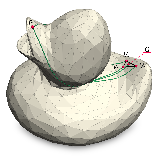
\includegraphics[height=2in]{figs/asd/fig2_a.png}
  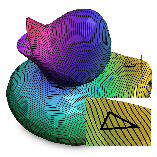
\includegraphics[height=2in]{figs/asd/fig2_b.png}\\
  \makebox[2in]{(a)}\makebox[2in]{(b)}\\
  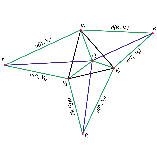
\includegraphics[height=2in]{figs/asd/fig2_c.png}
  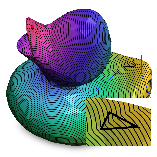
\includegraphics[height=2in]{figs/asd/fig2_d.png}\\
  \makebox[2in]{(c)}\makebox[2in]{(d)}\\
  \caption{Computing the single-source all-destination geodesic distances on a low-resolution mesh.
  (a) Let $p$ be the source point (also a mesh vertex) and $q$ a point inside a triangle $\bigtriangleup v_1v_2v_3$.
  (b) Using the saddle vertex graph, we can accurately compute the geodesic distances from $p$ to any mesh vertex.
  With the geodesic distances defined on each vertex, one can easily estimate the distances inside a triangle using linear interpolation.
  However, the interpolated distances have very low accuracy, since the distance is not a linear function.
  (c) The geodesic triangle unfolding method can significantly improve the accuracy.
  With known geodesic distances $d(p,v_i)$, $i=1,2,3$, we can unfold the geodesic triangles,
  $\bigtriangleup pv_2v_3$, $\bigtriangleup v_1pv_3$ and $\bigtriangleup v_1v_2p$, onto $\mathbb{R}^2$.
  Then the geodesic distance $d(p,q)$ is approximated by the minimal distance of three Euclidean distances $d(p_i,q)$.
  (d) The texture mapping reveals the high quality result by the GTU method.}
  \label{fig:SVGandGTU}
  \end{figure}

\subsection{Combination of SVG and GTU}
  Consider a triangle mesh $M=(V,E,F)$, where $V$, $E$ and $F$ are the set of vertices, edges and faces, respectively.
  A vertex $v$ is called \textit{saddle} if the sum of its interior angles exceeds $2\pi$.
  Mitchell et al.~\cite{Mitchell_Etc:1987} proved that a discrete geodesic path cannot pass through a spherical vertex
  unless it is an endpoint or a boundary point and the unfolded image of the path along any edge sequence is a straight line segment.

  The geodesic path $\gamma(v_i,v_j)$ between two vertices $v_i, v_j\in V$ is called direct, if it does not pass through any saddle vertices.
  Otherwise, it can be partitioned into several segments so that each segment is direct.
  Let $\Gamma=\{\gamma(v_i,v_j)|\gamma(v_i,v_j)~\text{is direct}, \forall v_i,v_j\in V\}$ denote the set of all direct geodesic paths on $M$.
  Then the saddle vertex graph associated to mesh $M$ is an undirected graph $G=(V,\Gamma)$.
  All the existing exact geodesic algorithms, such as the MMP algorithm~\cite{Mitchell_Etc:1987}, the ICH algorithm~\cite{Xin_Wang:2009},
  and most recently, the FWP-enhanced algorithm~\cite{fwp}, can be used to construct SVG.
  Ying et al.~\cite{Ying13SVG} observed that it is \textit{not} necessary to compute \textit{all} direct geodesic paths,
  in fact, a small subset of $\Gamma$ can lead to a pretty good result.
  Therefore, they suggested a simple-yet-effective heuristic to control the SVG size using a parameter $K$:
  for a vertex $v$, only the direct geodesic paths within a geodesic disk containing $K$ or less vertices are considered.
  They observed that a typical $K\in[50, 200]$ produces geodesic distances of accuracy $10^{-3}\sim 10^{-4}$, which are good for most applications.

  The SVG $(V,\Gamma)$ allows us to compute the geodesic distance between any pair of mesh vertices.
  To combine SVG and GTU, we take all mesh vertices as the samples, i.e., $m=n$.
  This strategy has three advantages:
  First, we totally avoid the construction of geodesic triangulation on $M$, since each $f\in F$ is a geodesic triangle.
  Second, we don't need to explicitly compute and store the \textit{entire} dense weighted graph for the GTU method,
  since the SVG method allows us to compute the geodesic distance between any pair of samples (i.e., vertices) on the fly.
  Third, as pointed out by Xin et al.~\cite{xin2012constant}, the larger the value of $m$, the higher the accuracy of the computed geodesic distance.
  The best accuracy of the GTU method is obtained by setting $m=n$.

  Now we are ready to compute the geodesic distance between arbitrary surface points $p,q\in M$.
  To ease presentation, we first address the simple case when one point, say $p\in V$, is a vertex, and the other $q\notin V$ is not.
  Let $\bigtriangleup v_1v_2v_3$ be the triangle containing $q$. See Figure~\ref{fig:SVGandGTU}(a).
  To compute the geodesic distance $d(p,q)$, we first apply the SVG method to compute geodesic distances $d(p,v_i)$, $i=1,2,3$.
  Note that the three geodesic distances together with three mesh edges $v_1v_2$, $v_2v_3$, $v_3v_1$, form three geodesic triangles.
  We unfold the geodesic triangles $\bigtriangleup pv_2v_3$, $\bigtriangleup v_1pv_3$ and $\bigtriangleup v_1v_2p$, onto $\mathbb{R}^2$,
  and obtain three images of $p$, namely, $p_1$, $p_2$ and $p_3$.
  Finally, the geodesic distance $d(p,q)$ is approximated by the minimal distance of three Euclidean distances $d(p_i,q)$.
  See Figure~\ref{fig:SVGandGTU}(c).

  The general case $p, q\notin V$ can be solved by unfolding both of the mesh triangles containing $p$ and $q$, respectively.
  Readers can refer to~\cite{xin2012constant} for the details.

\subsection{Improving the SVG Performance}

  SVG naturally links the discrete geodesic problem on polyhedral surfaces and the shortest path problem on graphs,
  since computing the geodesic distance between $p$ and $q$ is equivalent to finding a shortest path on the corresponding saddle vertex graph.
  Dijkstra's shortest path algorithm~\cite{dijkstra1959note} is a widely used technique for computing the shortest path.
  In the following, we review some fundamental concepts of the Dijkstra algorithm and its improvements.

  Let $G=(N,A)$ be an undirected graph, where $N$ and $A$ are the sets of nodes and arcs, respectively.
  Let $w_{ij}\geq 0$ be the non-negative weight of the arc $(n_i,n_j)$.
  To compute the shortest paths from a single node, say $n_1$, to all of the other vertices,
  the Dijkstra algorithm maintains a label vector $(d_1,d_2,...,d_{|N|})$ and a set of nodes $\mathcal{C}$, called the candidate list,
  starting with $d_1=0$, $d_i=\infty$ for $i\neq 1$, $\mathcal{C}=\{1\}$.
  The Dijkstra algorithm iteratively processes the nodes from the candidate list $\mathcal{C}$ and terminates when $\mathcal{C}$ is empty.
  Upon termination, each label $d_i$ is the shortest distance from the source $n_1$ to node $n_i$.

  The Dijkstra algorithm takes the node with the smallest label in the candidate list $\mathcal{C}$.
  Since each node enters and exits $\mathcal{C}$ exactly once, Dijkstra's algorithm takes $|V|$ iterations.
  The Dijkstra algorithm has many variants,
  which is distinguished by the data structures used to compute the minimal label node from $\mathcal{C}$.
  Examples include binary heap, Fibonacci heap, etc.

  The Dijkstra algorithm is known as a \textit{label setting} (LS) method, since the node removed from the list is permanently labeled and never enters the list again.
  Methods that do not follow this node selection policy are called label correcting (LC).
  These methods maintain a queue for the candidate list $\mathcal{C}$ and the nodes can enter and exit the queue in constant time $O(1)$.
  Therefore, selection of the node to be removed from $\mathcal{C}$ is faster than Dijkstra's algorithm, at the expense of multiple entrances of nodes in $\mathcal{C}$.

  We adopt the Small Label to the Front (SLF) scheme~\cite{bertsekas1993simple} for node insertion and the Large Label Last (LLL) scheme~\cite{Bertsekas96} for extraction:
  When a node $n_j$ enters the queue $\mathcal{C}$, its labels $d_j$ is compared with the label $d_i$ of the top node $n_i$ of $\mathcal{C}$.
  If $d_j\leq d_i$, node $n_j$ is entered at the top of $\mathcal{C}$; otherwise $n_j$ is entered at the bottom of $\mathcal{C}$.
  The top node $n_i$ exits the queue $\mathcal{C}$ if its label is less than a threshold;
  otherwise send $n_i$ to the bottom of $\mathcal{C}$.
  The threshold is usually set as the mean value of the labels of all the nodes in $\mathcal{C}$.

  The label setting algorithm performs at most one iteration per node, but requires some extra overhead (e.g., extracting the node with minimum label) per iteration.
  The label correcting methods, in contrast, takes more iterations than the Dijkstra algorithm, but the overhead per iteration is smaller.
  We evaluate the performance of the SLF-LLL based label correcting method on SVGs of a wide range of real-world models.
  As Table~\ref{table:timeperformance} shows, the label correcting driven SVG can almost double the runtime performance of the Dijkstra driven SVG.
  It is worth noting that the LC-enhanced SVG has an empirical $O(Dn)$ time complexity to compute the single-source-all-destination geodesic distances,
  since the graph has $O(Dn)$ edges and the overhead per iteration is $O(1)$.
  \begin{table}[htbp]
  \centering
  \begin{tabular}{|c|c|c|c|c|}
  \hline
  Method & Pre-computing time & Space & SSAD & Query points\\
  \hline
  \hline
  GTU~\cite{xin2012constant} & $O(mn^2\log n)$ & $O(m^2)$ & $O(n)$ & arbitrary\\
  \hline
  SVG~\cite{Ying13SVG} & $O(nK^2\log K)$ & $O(Dn)$ & $O(Dn\log n)$ & mesh vertices only\\
  \hline
  LC-SVG+GUT & $O(nK^2\log K)$ & $O(Dn)$ & empirical $O(Dn)$ & arbitrary\\
  \hline
  \end{tabular}
  \label{tab:complexity}
  \caption{Time and space complexities.
  $n$: \# of vertices; $m$: \# of sample points specified by the user;
  $K$: the size of geodesic disk containing the direct geodesic paths;
  $D$: model-dependent-but-resolution-insensitive constant;
  SSAD: single-source-all-destination.}
  \end{table}

\subsection{Geodesic Polar Coordinates}

  \begin{figure}[htbp]
  \centering
  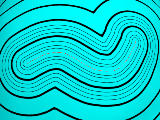
\includegraphics[width=0.45\textwidth]{figs/asd/parameterization3.png}
  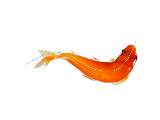
\includegraphics[width=0.45\textwidth]{figs/asd/parameterization4.png}\\	
  \makebox[0.45\textwidth]{(a) Geodesic offsets} \makebox[0.45\textwidth]{(b) Parameterization result}
  \caption{Geodesic polar coordinates.
  (a) Our LC-enhanced SVG method is able to compute the geodesic distances for curved sources.
  Each offset curve is then parameterized by arc-length.
  (b) The offset distance $\delta$ together with the normalized arc-length $\widehat{s}$ uniquely determine a point on the 3D surface.
  The geodesic polar coordinate system, formed by the 2-tuple $(\delta,\widehat{s})$,
  defines a bijective map between $\mathbb{R}^2$ and the patch on 3D surface.
  }
  \label{fig:offsets}
  \end{figure}
  A key component for computing the shape distribution is to map the 2D object onto 3D models.
  Global parameterization, adopted in the existing anisotropic sampling algorithm~\cite{li:anisotropic:2010}, is not a good choice,
  since global parameterization is computationally expensive and it also produces large distortion, which may lead to numerical issues and/or visual artifacts.
  A possible solution is the exponential map induced local parameterization, which builds a geodesic polar coordinate system on 3D surfaces.
  Given a \textit{smooth} surface $S$ and consider a point $p\in S$.
  Each tangent direction $\mathbf{v}\in T_{p}$ corresponds to a unique geodesic $\gamma_{\bf v}$ passing through $p$ in direction $\bf v$,
  i.e., $\gamma_{\bf v}(0)=p$ and $\gamma_{\bf v}'(0)=\bf v$.
  Thus, a point $q\in \gamma_{\bf v}$ can be represented by a 2-tuple $(\rho,\theta)$,
  where $\rho$ is the geodesic distance between $p$ and $q$, and $\theta$, the polar angle, corresponds to the tangent direction $\bf v$.
  Differential geometry can guarantee that on a sufficiently small neighborhood of $p$\footnote{When $\rho$ is less than the injective radius of $p$, the minimizing geodesic is unique,
  so that the geodesic distance $\rho$ and the polar angle can \textit{uniquely} determine a point in the neighborhood.},
  the exponential map is a diffeomorphism, i.e., both the function and its inverse are smooth.

  \textit{Discrete} exponential map has many applications in computer graphics and digital geometry processing, for example, surface decaling~\cite{Schmidt:2006:IDC:1141911.1141930},
  Possion disk sampling~\cite{DBLP:journals/tvcg/YingXS013}, intrinsic CVT computation~\cite{DBLP:journals/cad/WangYLXWGM015}, just name a few.
  Moreover, exponential map can be extended to a general setting, where the source is a curve~\cite{Sun:2013:TBI:2448196.2448221}.
  In spite of its popularity, the exponential map induced parameterization, in general, is not bijective due to two reasons:
  First, geodesics are not unique when their lengths exceed the injective radius.
  Consider two geodesic paths $\gamma_{\bf v_1}$, $\gamma_{\bf v_2}$ of equal length $\rho$ meet at a point $q$,
  then both $(\rho,\theta_1)$ and $(\rho,\theta_2)$ refer to the same point $q$.
  Second, as shown in~\cite{Ying13SVG}, when a geodesic path passes through a saddle vertex (whose cone angle is more than $2\pi$),
  it splits into many outgoing geodesic paths, meaning that all the outgoing geodesic paths share the same tangent direction.
  To fix the above-mentioned issues, Sun et al. \cite{Sun:2013:TBI:2448196.2448221} adopted a two-step strategy:
  They observed that the non-bijective issue occurs usually on part of the to-be-parameterized patch.
  Thus, they proposed a method for quickly detecting such regions.
  Then they computed a harmonic function to send these regions to rectangular domain.
  Since the target domain is convex, the harmonic map is guaranteed to be bijective.
  Schmidt \cite{CGF:CGF12045} applied Dijkstra's algorithm to spread out the local parameters and his method can parameterize self-intersecting strokes.

  Both Sun et al's method and Schmidt's method require local remeshing, which is a significant overhead, especially for the to-be-parameterized patch is big.
  In this section, we propose a simple-yet-effective method for computing the polar coordinates.
  Our method is completely integrated into the geodesic computation framework, and the induced parameterization is guaranteed to induce a bijective map.
  \begin{wrapfigure}{r}{2.5in}
  \centering
  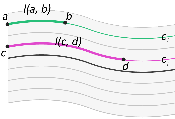
\includegraphics[width=2.45in]{figs/asd/para.png}
  \end{wrapfigure}
  Note that the combined SVG and GTU method can compute geodesic distances with both point sources and curve sources.
  Here we discuss the case of curve source, since the point source is a special case.
  Consider a curve ${c}_{s}$ as the source.
  The $u$-axis is along the source curve ${c}_{s}$ and $u$ values range $[0, 1]$ after the normalization by the length of ${c}_{s}$.
  Each geodesic offset curve is then parameterized by the arc-length to get the corresponding $u$ values.
  As shown in the above inset, we define ${c}_{i}$ and ${c}_{j}$ are two isoline curves,
  ${u}_{a}$, ${u}_{c}$ are the two corresponding start points of curve ${c}_{i}$ and ${c}_{j}$, ${u}_{b}$, ${u}_{d}$ are two arbitrary points on curve ${c}_{i}$ and ${c}_{j}$.
  The $u$ value at point ${u}_{b}$ is $\frac{l({u}_{a},{u}_{b})}{l({c}_{i})}$ and is $\frac{l({u}_{c},{u}_{d})}{l({c}_{j})}$ at point ${u}_{d}$,
  where $l({u}_{c},{u}_{d})$ represents the length of curve between ${u}_{c}$ and ${u}_{d}$.
  Note that the $u$ values of each point are only related to the arc-length on the corresponding iso-curve,
  meaning that the polar coordinate is guaranteed to be bijective.
  In contrast to~\cite{Sun:2013:TBI:2448196.2448221}, our method does not solve any linear system, thus, it is numerically stable and efficient.
  Computational results show that our method is up to 10 times faster than~\cite{Sun:2013:TBI:2448196.2448221}.
  See Figure~\ref{fig:parameterization_compare}.
  \begin{figure}[!htb]
  \centering
  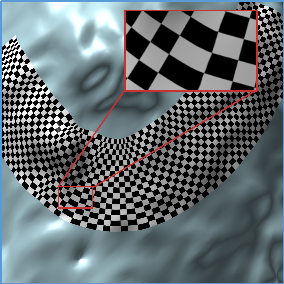
\includegraphics[width=0.45\textwidth]{figs/asd/sq_parameterization_result_enlarge.png}
  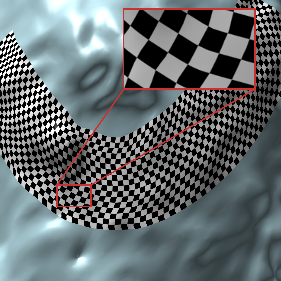
\includegraphics[width=0.45\textwidth]{figs/asd/wxn_parameterization_result_enlarge.png}
  \makebox[0.45\textwidth]{(a) Extended exponential map~\cite{Sun:2013:TBI:2448196.2448221}}
  \makebox[0.45\textwidth]{(b) Our result}
  \caption{Comparison with extended exponential map~\cite{Sun:2013:TBI:2448196.2448221}.
  Our result has comparable quality as Sun et al.'s method~\cite{Sun:2013:TBI:2448196.2448221}.
  Since their method computes a harmonic map to fix the non-bijective issue of the exponential map,
  it is more computationally expensive than ours.
  It takes their method 1.7 seconds to parameterize the 10K-vertex patch, whereas our method spends only 0.18 seconds.}
  \label{fig:parameterization_compare}
  \end{figure}




\section{Parallel Distribution of Anisotropic Shapes}

\subsection{Motivation}

A simple algorithm for distributing shapes is the traditional dart throw method. Dart throw method can generates uniformly and randomly distributed samples but is not efficient. It throws a large number of darts and only accept a small percentage of them.
And it's not easy to parallel. Thus we present an improved algorithm inspired from Ying et al.~\cite{DBLP:journals/tvcg/YingXS013}. We first randomly generate a large number of points on the surface following Osada et al.~\cite{Osada:2002:SD:571647.571648}'s algorithm, which are unbiased and insensitive to mesh tessellation. Then we start to integrate the vector field from the point to both direction to get a large number of curves. The curve serve as the center line of geodesic polar coordinates which is used to parameterize the shape on surface. Once a curve is accepted, we use the curve as source and compute a geodesic region with distance $2r$. The shapes with distance larger than $2r$ are guaranteed to be free of conflicts. While shapes within 2r may or may not conflict. Then we use a technique introduced in Section~\ref{sec:single_shape_distribution} called \textit{Minimum Safe Distance
Table} to check conflicts and rejected all the shapes which have conflicts. The algorithm terminates when all predefined curves have been processed. To parallelize the algorithm, we assigning a \textit{unique random} value to each shape, which represents the priority of the shape. Then the candidate shapes can be processed by multiple threads at the same time. Each thread checks the collision within a shape's neighbors. The shape with the higher priority will be accepted.



  \begin{figure*}
  \centering
  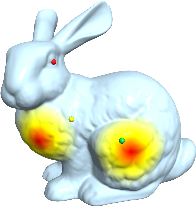
\includegraphics[width=0.24\textwidth]{figs/asd/pipeline_singularity_density.png}
  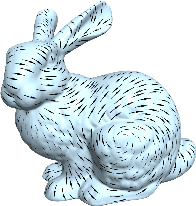
\includegraphics[width=0.24\textwidth]{figs/asd/fig5_c_vector_field.png}
  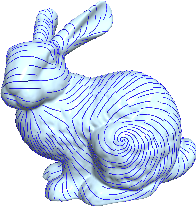
\includegraphics[width=0.24\textwidth]{figs/asd/pipeline_curves40.png}
  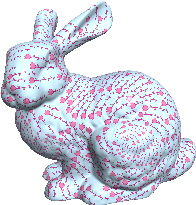
\includegraphics[width=0.24\textwidth]{figs/asd/pipeline_flowerlong_40.png}\\
  \makebox[0.35\textwidth]{(a) Density control \& singularities}
  \makebox[0.2\textwidth]{(b) Vector field}
  \makebox[0.2\textwidth]{(c) Central lines}
  \makebox[0.2\textwidth]{(d) Result}  \\
  \caption{Algorithmic pipeline of single-class shape distribution.
  (a) User specifies a scalar field to control the shape density and the locations of singularities and their indices.
  (b) We adopt Crane et al.'s method~\cite{crane2010trivial} to compute the vector field which controls the shape orientation.
  (c) Our method automatically determines the locations, sizes and orientations of the 2D objects.
  Each blue curve represents the central line of one object.
  (d) Thanks to the minimal safe distance table, all distributed objects are guaranteed to be collision-free.}
\label{fig:pipeline}
\end{figure*}

\subsection{User Input}

Our algorithm allows the user to control the density and the orientation of each class. The user can specify density field by choosing the density center and specify vector field by choose singularities. Then we will generate a vector field using Crane et at.'s method~\cite{crane2010trivial}. We distribute shapes along the vector field adaptively and anisotropically. Please refer to Figure~\ref{fig:pipeline} for the algorithm overview.

After density field is generated, we can get a user specified spatial variety function $g(\star)\rightarrow [1, M]$, then an adaptive distribution is defined. We need to compute a geodesic region with radius $(1+M)r$ for each point. For
point $p$ and $q$, we use the new min safe distance(the detail of min safe distance will explained in Section~\ref{sec:single_shape_distribution}):
\[ \frac{g(p) + g(q)}{2}D(\alpha, \beta) \].

For multi-class, user can specify $g_i(\star) \rightarrow [1, M_i]$
for each shape. We need to compute a geodesic disk with radius $r +
\max(M_ir, r_m)$. we use \[ \frac{g_i(p) + g_i(q)}{2}D_{i,i}(\alpha,
\beta) \]  if $p,q$ are the same class. We use $D_{i,j}(\alpha,
\beta)$ directly if $p, q$ are different classes.

To make the surface shape distribution organized and controllable, we use the user-controlled vector field to control the directions of shapes. We adopted a globally optimal vector field generalization method from Crane~et al.~\cite{crane2010trivial}. Our system allows the user to set singularities and direction constraints on the surface directly, as shown in figure ~\ref{fig:pipeline}(a). Each singularity has an index indicating the number of full rotations along a small loop around the vertex. The sum of index of singularities of a vector field on 3D mesh is equal to the Euler characteristic~\cite{crane2010trivial}. The user also can sketch stokes on the surface to specify the desired vector filed direction. According to the stokes' direction of corresponding faces, we fix the vector field direction of the specific area. The vector field is then computed by solving a convex optimization problem with linear constraint.

\subsection{Algorithm}
We use parallel sampling algorithm to generate a set of shapes centered as the curves following the vector field.
Here we describe how to generate curves following the distance field. Each time we throw a point on the triangle mesh $M$, we trace the curve starting from each point along the vector field. We use curve integration method, starting from a surface point, we walk along the direction field on the triangle which the point belong to. When we encounter an edge, we set the intersection point of the tracing curve and the edge as the new starting point. We repeat this until the length of the curve reach a given length $l_{max}$. The resulting curves are piecewise linear polylines on the mesh $M$.

\subsubsection{Single-class Shape Distribution} \label{sec:single_shape_distribution}

\begin{figure}[htbp]
\centering
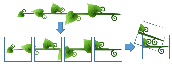
\includegraphics[width=0.8\textwidth]{figs/asd/shape_cut_1.png}
\caption{For long shapes, we divide it to several parts and test the intersection seperatly.}
\label{fig:shape_cut}
\end{figure}

A 2D object $S$ is mapped to the surface along a curve,
to make sure they do not intersect each other we need an efficient method
to check the conflict. For long shapes, we splite the long shape into equal size parts and check each part using precomputed distance table. Fig.~\ref{fig:shape_cut} gives a brief illustration.

Now we introduce the details of distance table technique.
Given a 2D object $S$, we compute the smallest covering circumcircle
$\odot(c,r)$, where $c$ is the center and $r$ is the radius (see
Figure~\ref{fig:singleshapedemo}). The circle can be computed in
linear time using~\cite{Megiddo:1982:LAL:1382436.1382771}. We then
choose a ray $L$ from the center $c$ to a fixed direction as the
polar axis. Clearly, objects that are $2r$ apart (distance between
their center points) are guaranteed to be free of conflicts.
However, objects within $2r$ may or may not conflict, depending on
their orientations.

  \begin{figure}[!htb]
  \centering
  \fbox{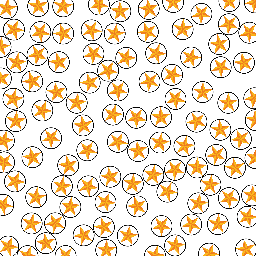
\includegraphics[width=0.4\textwidth]{figs/asd/star_poissondisk_103pts_withcircle.png}}
  \fbox{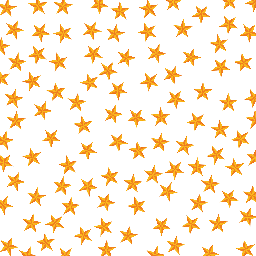
\includegraphics[width=0.4\textwidth]{figs/asd/star_poissondisk_103pts_withoutcircle.png}}\\
  \makebox[0.4\textwidth]{103 stars}\\
  \fbox{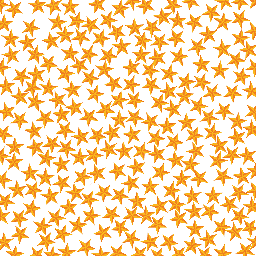
\includegraphics[width=0.4\textwidth]{figs/asd/star_ourmethod_221pts.png}}
  \fbox{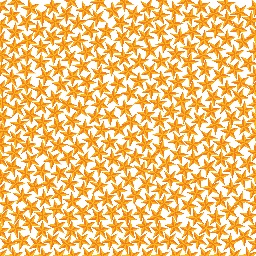
\includegraphics[width=0.4\textwidth]{figs/asd/star_dense_333pts.png}}\\
  \makebox[0.4\textwidth]{221 stars} \makebox[0.4\textwidth]{333 stars}
  \caption{Comparison with Poisson disk sampling.
  Row 1: Poisson disk sampling considers each sample as a disk and does not allow overlapping disks.
  Row 2: Our method allows a more dense distribution than Poisson disk sampling, as long as the stars are not overlapping.
  }
  \label{fig:comparetopoissondisk}
  \end{figure}


To efficiently determine whether or not two objects conflict, we
pre-compute a look up table, named \textit{Minimum Safe Distance
Table}, or MSDT for short.

As shown in Figure~\ref{fig:singleshapedemo}(right), the relation
between two objects $A$ and $B$ is determined by the distance
between two center points $d(c_A,c_B)$ and the orientations of each
object. The latter is characterized by the angles between the polar
axis and the line $c_Ac_B$, denoted by $\alpha$ and $\beta$,
respectively.

We uniformly divide $[0, 2\pi)$ into $D$ intervals, and build a $D
\times D$ look up table. For each pair of angles $\{\alpha,
\beta\}$, the entry $D(\alpha,\beta)$ is the minimum distance
between the center points that guarantees no conflict, which is
computed as follows:

If the object is a 2D polygon with $e$ edges, we can check the
polygon intersection in $O(e^2)$ time. Thus, the \textit{Minimum
Safe Distance} $D(\alpha, \beta)$ can be found by the binary search
of $[0, 2r]$ in $O(D^2 e^2 \log r)$ time and with $O(D^2)$ space.

If the object is a 2D image with $b$ boundary pixels, we check each boundary pixel of shape B. If any
boundary pixel locates inside shape A, the two shapes are
conflicted. we can test whether two objects are conflicted in $O(b)$
time.

\begin{figure}[htbp]
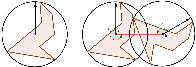
\includegraphics[width=0.9\textwidth]{figs/asd/singleshapedemo.png}
\caption{Left: circumcircle of shape. Right: The minimum safe distance between two shapes (red line).} \label{fig:singleshapedemo}
\end{figure}


  Putting it all together, the construction of MSDT takes $O(D^2 b \log r)$ time and occupies $O(D^2)$ space.

Let $C$ be the center-point of each shape, and vector
$\overrightarrow{CO}$ be the orientation. During the shortest path computation using SVG, we can unfold point $O$ together with the center $C$.
Thus, the angles $\{\alpha, \beta\}$ could be computed.

Our algorithm can compute $(\alpha, \beta, d_g)$ for each point
when computing the geodesic polar coordinates. Thus it's quite efficient and didn't requite additional computation cost.

The pseudo-code in algorithm~\ref{alg:shape_distribution} describes our distribution algorithm.

\begin{algorithm}[htbp]
\caption{Parallel Single Shape Distribution}
\begin{algorithmic}
\State $D \gets$ Minimum Safe Distance table.
\State $S \gets$ a dense random curve set
\State // The orientation of each
curve is guided by user specified vector field.
\State random\_shuffle($S$);
\State // now, consider $S$ as a queue of dart throwing curves.
\State
\textbf{foreach} $S_i$ \textbf{in}
$S$ \textbf{do} $S_i.myIndex \gets +\infty$
\State $curveOrder \gets0$
\State $result \gets \emptyset$
\State
\State \textcolor{blue} {foreach parallel thread do:}
\State \textbf{while} $S$ is not empty \textbf{do}
\State ~~~~\textcolor{red}{atomic} $t \gets curveOrder ++$
\State ~~~~//$t$ gets the value of $curveOrder$, and $curveOrder$ was increased by 1.
\State ~~~~\textcolor{red}{atomic} $p \gets S.pop\_front()$
\State ~~~~$p.myIndex \gets t$
\State ~~~~$\{w\} \gets$ use \textit{label correcting} algorithm to compute geodeisc region centered at curve $c$ with radius $2r$
\State ~~~~$isAccepted \gets true$
\State ~~~~\textbf{foreach} $w_i$ \textbf{in} $\{w\}$
\State ~~~~~~~~\textbf{if} $w_i.d_g < D[w_i.\alpha][w_i.\beta]$   $w_i.myIndex < p.myIndex$ \textbf{then}
\State ~~~~~~~~~~~~$isAccepted \gets false$
\State ~~~~~~~~~~~~\textbf{break foreach loop}
\State ~~~~~~~~\textbf{end if}
\State ~~~~\textbf{end for}
\State ~~~~\textbf{if} $isAccepted$ \textbf{then}
\State ~~~~~~~~\textcolor{red}{atomic} $result.push(c)$
\State ~~~~~~~~\textbf{foreach} $w_i$ \textbf{in} $\{w\}$
\State ~~~~~~~~~~~~\textcolor{red}{atomic} remove $w_i$ from $S$
\State ~~~~~~~~\textbf{end for}
\State ~~~~\textbf{end if}
\State \textbf{end while}
\State \textcolor{blue}{end thread}
\State
\State output $result$
\end{algorithmic}
\label{alg:shape_distribution}
\end{algorithm}



\subsubsection{Multi-Class Shape Distribution}

Our method is different from the multi-class blue noise sampling in~\cite{Wei:2010:MBN:1833351.1778816},
since we do not allow overlapped shapes.

In multi-class case, for a group of $k$ shapes $\{c_1, c_2, \ldots,
c_k\}$, we have to compute $k \choose 2$ different classes MSD table
and $k$ same class MSD table. thus, the time complexity is $O(k^2
D^2 b \log{r})$, takes $O(k^2 D^2)$ memory space.

algorithm input: vector field for each class $O_i$, target number of
each class $N_i$.

Similar like single shape distribution, we generate a dense point
set. Each point are specified to a shape. A point has a probability
$p_i$ to be $i$-th shape. $p_i$ is defined as:
\[ p_i \gets \frac{N_iA_i}{\sum_{j=1}^{k}{N_jA_j}} \]
where $A_i$ is the area of $i$-th shape.

let $r_i$ be the circumradius of $i$-th shape, and $r_m \gets
\max{r_i}, i = 1 \ldots k$. for each point of shape $i$, we compute
a geodesic disk with radius $r_i + r_m$, and collect all neighbor
points. Then check the MSD by looking up the table $D_{i,\star}(\alpha,
\beta)$


\section{Experimental Results}

  \noindent\textbf{Performance.} We implement the algorithm in C++ and test it on an Intel Xeon quad-core CPU at 2.66GHz.
  Thanks to the nice parallel structure of our method, we also use OpenMP to parallelize our algorithm so that it can take the advantage of all CPU cores.
  We observe that our parallel implementation on a quad-core CPU is up to 3 times faster than that of a single-core
  and it allows interactive manipulation on 3D models with 100K faces.
  See Table~\ref{table:shape_distribution_time} for running time performance and the accompanying video demonstration.
  Figures~\ref{fig:kitten_density}, \ref{fig:multiclass} and~\ref{fig:moreresults} demonstrate our results on single-class and multi-class shape distribution.

%  Our method allows the user to directly specify the location and index of singularities as well as the scalar field for density control.
%  See Figure~\ref{fig:pipeline}.
%  The vector filed is computed using Crane et al.'s method~\cite{crane2010trivial}.
%  Then the shape distribution is generated efficiently and the user can interactively edit the vector field and density until satisfied.
%  Below there are some time comparison and single and multi-class shape distribution results.

  \begin{table}[htbp]
  \centering
  \caption{Performance of geodesic algorithms.
  The ICH algorithm computes the exact geodesic distances, whereas the SVG method and our LC-enhanced SVG+GTU method compute the approximate distances.
  We set $K=50$ for constructing the SVG.
  $\varepsilon$: mean relative error of our method and the SVG method.
  Columns 3 to 5 report the running time (in seconds) of the geodesic algorithms.
  }
  \begin{tabular}{ | l | c | c | c | c | c | }					
  \hline
  Model & $|V|$ 	& $T_{ICH}$  & $T_{SVG}$	& $T_{our}$ 	& $\varepsilon$ 	 \\ \hline		
  \hline
  Torus & $200K$  						& 28.64    & 0.20  	& 0.09  			& 0.15\%			 \\ \hline	
  Fertility & $400K$ 					& 49.47    & 0.37  	& 0.21  			& 0.14\%			 \\ \hline	
  Kitten & $548K$						& 93.85    & 0.48  	& 0.30  			& 0.16\% 			 \\ \hline	
  Bimba & $800K$ 						& 125.03   & 0.70  	& 0.38  			& 0.13\% 			 \\ \hline	
  Dragon & $1.28M$ 						& 266.38   & 1.09  	& 0.60  			& 0.20\% 			 \\ \hline					 
  \end{tabular}%	
  \label{table:timeperformance}
  \end{table}

  \begin{table}[htbp]
  \centering
  \caption{Mesh complexity and running time performance.
  $T_1$ and $T_4$: running time (in seconds) on a quad-core CPU using a single core and all cores, respectively.}
  \begin{tabular}{ | l | c| c | c | c |  c | }					
		\hline
		Model  & $|F|$ & \# of 2D shapes & $T_1$ & $T_4$ \\ \hline		
		Bump Sphere & 50K  						& 458    & 3.1  	& 1.1  			 			 \\ \hline	
		Bunny  & 80K	 					&  561   & 4.2  	& 1.4  					 \\ \hline	
		Fertility & 400K 				& 1,150    & 8.1  	& 2.9  			 			 \\ \hline	
		Kitten & 250K 						& 864   & 9.5  	& 3.7  			 			 \\ \hline	
  \end{tabular}%	
  \label{table:shape_distribution_time}
  \end{table}

%\subsection{Examples with single and multiple classs}

  \begin{figure}[htb]
  \centering
  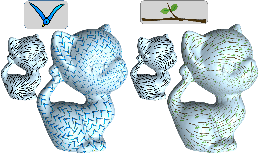
\includegraphics[width=0.8\textwidth]{figs/asd/kitten_singleclass_density.png}
  %%\includegraphics[height=2in]{figs/asd/amphamo_singleclass.png}
  %%\includegraphics[height=2in]{figs/asd/bunny_singleclass.png}\\
  \caption{Single-class shape distribution on the Kitten model with different density and texture. }
  \label{fig:kitten_density}
  \end{figure}

  \begin{figure}[htb]
  \centering
  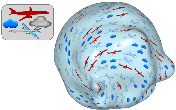
\includegraphics[width=0.6\textwidth]{figs/asd/multiclass_aotu.png}\\
%%\includegraphics[height=2in]{figs/asd/amphamo_singleclass.png}
%%\includegraphics[height=2in]{figs/asd/bunny_singleclass.png}\\
  \caption{Multi-class shape distribution on a bumpy sphere with 50K faces.}
  \label{fig:multiclass}
  \end{figure}

  \noindent\textbf{Robustness.} Our method is intrinsic since both the collision detection and shape distribution depend on the metric only.
  Thanks to the intrinsic nature of the geodesic algorithms~\cite{Ying13SVG,xin2012constant},
  our method is insensitive to mesh resolution and tessellation.
  See Figure~\ref{fig:bimba_robust} for our results on the Bimba model with various resolutions.

  \begin{figure}
  \centering
  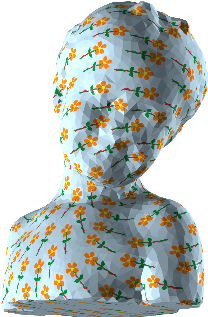
\includegraphics[width=0.3\textwidth]{figs/asd/bimba_nf7k_flower.png}
  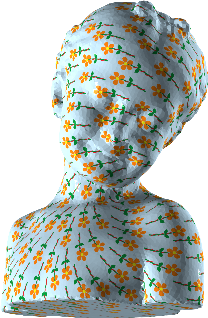
\includegraphics[width=0.3\textwidth]{figs/asd/bimba_nf30k_flower.png}
  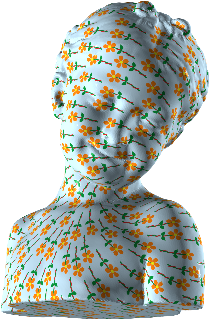
\includegraphics[width=0.3\textwidth]{figs/asd/bimba_nf149k_flower.png}\\
  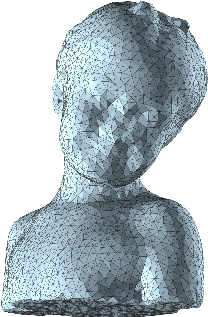
\includegraphics[width=0.3\textwidth]{figs/asd/bimba_nf7k_wireframe.png}
  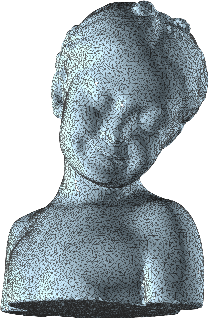
\includegraphics[width=0.3\textwidth]{figs/asd/bimba_nf30k_wireframe.png}
  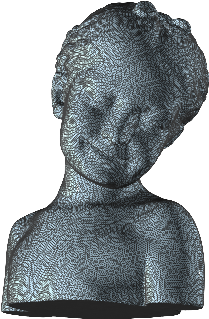
\includegraphics[width=0.3\textwidth]{figs/asd/bimba_nf149k_wireframe.png}\\
  \makebox[0.3\textwidth]{7K faces}\makebox[0.3\textwidth]{30K faces}\makebox[0.3\textwidth]{150K faces}
  \caption{Our method works well on the Bimba model with various resolutions. }
  \label{fig:bimba_robust}
  \end{figure}


  \noindent\textbf{Comparison to \cite{li:anisotropic:2010}.} Our method and the anisotropic blue noise sampling method~\cite{li:anisotropic:2010} differ in 4 aspects:
  First, their method is mainly designed for the 2D problem.
  Although it can be extended to 3D surfaces via global parameterization, computing a high quality parameterization for high-genus model is technically challenging.
  Our method is based on local parameterization, which can be computed efficiently on the fly.
  Therefore, our method can be applied to models of arbitrary geometry and topology.
  Second, their method is based on the dart throwing technique, which is a sequential process.
  It is hard to extend the existing parallelization techniques (such as the phase group method~\cite{Wei:2008:PPD:1399504.1360619}) to anisotropic setting,
  since anisotropy poses a challenge in domain partition.
  Third, their method abstracts the anisotropic shapes by bounding ellipses so that collision detection and quality evaluation can be done in an analytical manner.
  However, ellipse is not an effective representation if the 2D shape has a highly concave boundary.
  As a result, their method may produce a distribution which is far from maximal.
  Thanks to the minimal safe distance table, our method can faithfully keep the geometry of the 2D shapes hereby allow a much denser distribution.
  See Figure~\ref{fig:hawk}.
  Last but not the least, their method supports single-class sampling only, whereas our method can compute multi-class shape distribution.

  \begin{figure}[htbp]
  \centering
  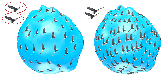
\includegraphics[width=0.8\textwidth]{figs/asd/conflict_compare.png}\\
  \makebox[0.5\textwidth]{(a) Li et al.'s result}\makebox[0.5\textwidth]{(b) Our result }
  \caption{Comparison to \cite{li:anisotropic:2010}.
  The 2D Eagle shape is highly concave, so a simple bounding ellipse cannot capture its geometric features.
  As a result, requiring non-overlapping ellipses is very pessimistic.
  Li et al.'s method~\cite{li:anisotropic:2010} can distribute only 115 shapes. Obviously, the distribution is not maximal.
  Our method produces a much more dense distribution, containing 224 eagles,
  since it allows overlapping ellipses as long as the adjacent eagles do not collide.}
  \label{fig:hawk}
  \end{figure}

  \begin{figure}[htb]
  \centering
  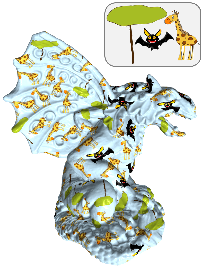
\includegraphics[height=4in]{figs/asd/gargoyle.png}
  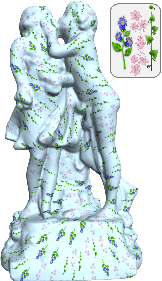
\includegraphics[height=4in]{figs/asd/sculpture.png}\\
  \caption{More results.}
  \label{fig:moreresults}
  \end{figure}

\section{Conclusion}
  This paper presents a practical method for computing anisotropic 2D shape distribution on arbitrary 2-manifold meshes with user control.
  Our method has several advantages:
  First, unlike the existing sampling approaches, which usually assume the 2D objects are isotropic and of simple geometry,
  our method applies for complex 2D objects and can guarantee the distribution is conflict-free, which is a critical constraint in many applications.
  Second, it is able to compute multi-class shape distribution and can also support maximal distribution so that no additional shapes can be inserted.
  Third, our method does not require global parameterization of the input 3D mesh.
  Instead, it compute local parameterization on the fly using geodesic polar coordinates, which has little computational cost.
  Therefore, our method can be applied to models of complicated geometry and topology.
  Last but not the least, our method has a natural parallel structure, and can be implemented on multi-core CPUs.
  Experimental results on a wide range of 3D models and 2D anisotropic shapes demonstrate the good performance as well as the effectiveness of our method.


